% Embedded animations in Beamer
\documentclass{beamer}
% Theme choice
% \usetheme{EastLansing}
\usepackage{sid}
% Required package
\usepackage{animate}
\usepackage{amsmath}
\usepackage{outlines}
\usepackage{bibentry}
\usepackage{chronology}
\nobibliography*
% \usepackage[backend=biber]{biblatex}

\usepackage{xr}
\externaldocument{../ch-introduction}
\externaldocument{../ch-literature}
\externaldocument{../ch-simulation}
\externaldocument{../ch-inversion}
\externaldocument{../ch-results}
\externaldocument{../ch-conclusion}
\externaldocument{../ch-appendices}
\graphicspath{{/Users/liamrobinson/Documents/PyLightCurves/docs/build/html/_images}}

\title[]{Light Curve Simulation and Shape Inversion for Human-Made Space Objects}
\author[]{Liam Robinson}
\institute{Purdue Space Information Dynamics Group}
\date{11/13/2023}

% ---------------------------------------------------------------
\begin{document} 
% Configuration
{
    % \usebackgroundtemplate{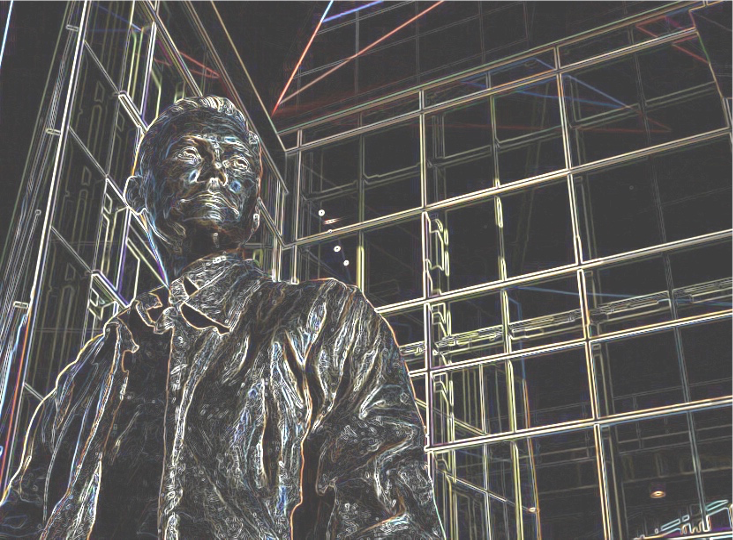
\includegraphics[decodearray={0.3 1.5 0.3 1.5 0.3 1.5},width=\paperwidth,height=\paperheight]{figs_config/neil.png}}
    \usebackgroundtemplate{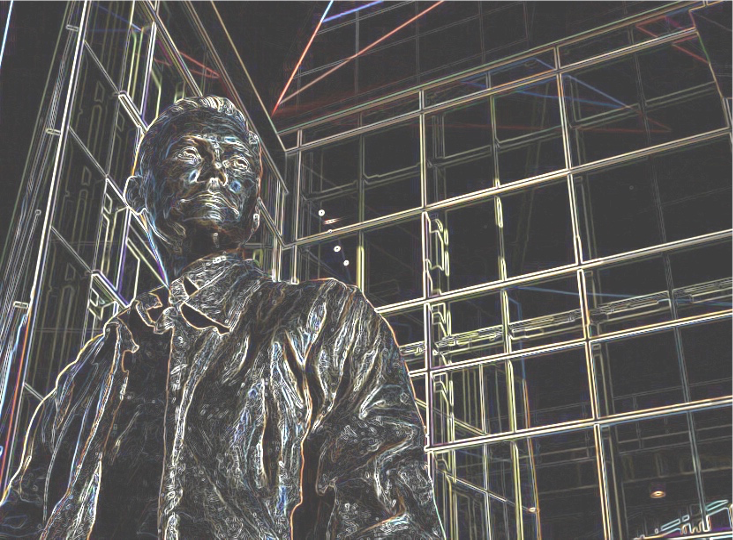
\includegraphics[decodearray={-0.3 0.5 -0.3 0.5 -0.3 0.5},width=\paperwidth,height=\paperheight]{figs_config/neil.png}}
    \begin{frame}[plain]
    \titlepage
    \end{frame}
}
% Set up outline 
\AtBeginSection[]
{
\begin{frame}{Outline}
    \tableofcontents[currentsection]
\end{frame} 
}

\section{Introduction}

\begin{frame}{Motivation}
    \begin{outline}
        \1 Space is becoming more crowded
        \1 We have an imperfect understanding of the space environment
        \1 Understanding the shape of debris objects is important for orbit propagation and active removal
    \end{outline}

    \begin{figure}
        \centering
        \includegraphics[width=0.9\textwidth]{sphx_glr_propagate_catalog_001.png}
        \label{fig:debris}
        \caption{Publicly tracked objects in 2000 and 2023}
    \end{figure}
\end{frame}

\begin{frame}{Research Objectives}
    \begin{outline}
        \1 Developing a high-fidelity light curve simulation framework to simulate the physics of real measurements
        \1 Adapting direct shape inversion techniques for human-made space objects
        \1 Designing a new method for inverting shape with noisy measurements and estimating nonconvex geometry
    \end{outline}
\end{frame}

\begin{frame}{State of The Art: Simulation}

    \begin{outline}
        \1 Light curve simulation literature often assumes:
        \2 Uniform material properties
        \2 Self-shadowing is negligible
        \2 Object geometry is simple \cite{cabrera2021}
        \2 Measurement noise is negligible or Gaussian \cite{fan2020thesis}
    \end{outline}
\end{frame}

\begin{frame}{State of The Art: Shape Inversion}

    \begin{outline}
        \1 Direct shape inversion
        \2 Require \textit{a priori} knowledge of material properties and attitude
        \2 Highest fidelity shape estimates
        \1 Filter-based methods
        \2 Attempt to estimate shape and attitude simultaneously
        \2 Limited to simple geometries
        \1 Deep learning
        \2 Trains models to classify objects by their light curves
        \2 Unpredictable behavior outside the training set
    \end{outline}

    This work presents improvements to direct shape inversion
\end{frame}

\begin{frame}{Direct Inversion Literature Timeline}
    Asteroid Inversion
    \begin{chronology}[4]{2000}{2022}{\textwidth}
        \event{1997}{Russell (1906) \cite{russell1906}}
        \event{2000}{Kaasalainen \cite{kaasalainen2000, kaasalainen2001, kaas2002models}}
        \event{2003}{Durech \cite{durech2003}}
        \event{2014}{Yu \cite{yu2014shape}}
        \event{2022}{Chng \cite{chng2022}}
    \end{chronology}

    Human-made Object Inversion
    \scriptsize{
    \begin{chronology}[4]{2000}{2022}{\textwidth}
        \event{1998}{Ikeuchi (1981) \cite{ikeuchi1981}}
        \event{1999}{Little (1985) \cite{little1985}}
        \event{2003}{Gardner \cite{gardner2003}}
        \event{2007}{Hall \cite{hall2007separating}}
        \event{2014}{Bradley \cite{bradley2014}}
        \event{2019}{Fan \cite{fan2019}}
        \event{2020}{Fan \cite{fan2020thesis} and Friedman \cite{friedman2020}}
        \event{2021}{Cabrera \cite{cabrera2021} and Fan \cite{fan2021}}
        \event{2022}{Robinson \cite{robinson2022} and Friedman \cite{friedman2022}}
    \end{chronology}
    }
\end{frame}

\section{Light Curve Simulation}

\begin{frame}{Attitude Motion}
    \begin{outline}
        \1 Environmental torques do exist on orbit, but can be neglected on the scale of minutes to hours
        \1 Torque-free attitude motion for rigid bodies is described by Euler's equations of motion for an inertia tensor $J$ and body frame angular velocity $\mathbf{\omega}$:
        \begin{equation*}
            \dot{\mathbf{\omega}} = J^{-1} \left[ \left(J \mathbf{\omega} \right) \times \mathbf{\omega} \right]
        \end{equation*}
        \1 These EOMs are integrated with a quaterion $\mathbf{q} = \left[q_1, q_2, q_3, q_4 \right]^T$ to track the orientation of the body in inertial space:

        \begin{equation*}
            \left[\begin{matrix}\dot{\epsilon_1}\\\dot{\epsilon_2}\\\dot{\epsilon_3}\\\dot{\epsilon_4}\\\end{matrix}\right]
            =
            \frac{1}{2}\left[\begin{matrix}\epsilon_4&-\epsilon_3&\epsilon_2&\epsilon_1\\\epsilon_3&\epsilon_4&-\epsilon_1&\epsilon_2\\-\epsilon_2&\epsilon_1&\epsilon_4&\epsilon_3\\-\epsilon_1&-\epsilon_2&-\epsilon_3&\epsilon_4\\\end{matrix}\right]
            \left[\begin{matrix}\omega_1\\\omega_2\\\omega_3\\0\\\end{matrix}\right].
        \end{equation*}
    \end{outline}
\end{frame}

\begin{frame}{Types of Torque-Free Motion}
    \animategraphics[loop,width=4cm]{30}{imgs/sphx_glr_vis_attitude_motion_001/}{0}{199}
    \animategraphics[loop,width=4cm]{30}{imgs/sphx_glr_vis_attitude_motion_002/}{0}{199}
\end{frame}

\begin{frame}{Bidirectional Reflectance Distribution Functions (BRDFs)}
    \begin{outline}
        \1 BRDFs describe how light is reflected from a surface
        \2 $f_r(L,O)$ describes the fraction of incident light $L$ reflected in the direction of an observer $O$
        \1 Many formulations exist, but to be relevant to this work, they must \cite{montes2012}:
        \2 Conserve energy for all $L$:
        \[
            \int_{O \in \mathbb{S}^2} f_r(L, O) \: d\mathbb{S}^2 \leq 1
        \]
        \2 Be nonnegative: $f_r(L, O) \geq 0$ for all $L$ and $O$
        \2 Be reciprocal: $f_r(L, O) = f_r(O, L)$ for all $L$ and $O$
        \1 Popular relevant BRDFs include:
        \2 Lambertian \cite{montes2012}
        \2 Phong \cite{phong1975}
        \2 Cook-Torrance \cite{cook1982}
    \end{outline}
\end{frame}

\begin{frame}{BRDFs in Action}
    \begin{figure}
        \centering
        \includegraphics[width=0.8\textwidth]{sphx_glr_brdf_renders_002_2_00x.png}
        \label{fig:brdfs}
        \caption{BRDFs implemented for this work}
    \end{figure}
\end{frame}

\section{Direct Shape Inversion}

\section{Discussion}

\section{Conclusion}

\begin{frame}{The Earth}
center

\begin{center}
    \animategraphics[loop,width=4cm,draft]{30}{imgs/sphx_glr_plot_earth_001/}{0}{99}
\end{center}
\end{frame}

\begin{frame}{EGI Optimization}
    Equation 
\end{frame}

\bibliographystyle{unsrt}
\bibliography{{/Users/liamrobinson/Documents/PyLightCurves/docs/source/_static/refs.bib}}

\end{document}
